\documentclass[conference]{IEEEtran}
% \IEEEoverridecommandlockouts

\usepackage{cite}
\usepackage{amsmath,amssymb,amsfonts}
\usepackage{algorithmic}
\usepackage{graphicx}
\usepackage{textcomp}
\usepackage{xcolor}
\usepackage{tabularx}
\usepackage{array}
\usepackage{subcaption}
\usepackage{booktabs}
\usepackage{multirow}

\newcolumntype{Y}{>{\raggedright\arraybackslash}X}

\def\BibTeX{{\rm B\kern-.05em{\sc i\kern-.025em b}\kern-.08em
    T\kern-.1667em\lower.7ex\hbox{E}\kern-.125emX}}
\begin{document}

\begin{titlepage}
    \centering

    {\Huge\bfseries RES: A modular pipeline to recognise, encode and select relevant facts from clinical notes\par}
    \vspace{2cm}

    {\large
    A dissertation submitted in partial fulfilment of\par
    The requirement for the degree of\par
    MASTER OF SCIENCE in Artificial Intelligence\par
    in\par
    The Queen’s University of Belfast\par
    by\par
    Conor Brown\par
    4th September 2026
    }
\end{titlepage}


\title{RES: A modular pipeline to recognise, encode and select relevant facts from clinical notes\\}



\maketitle

\begin{abstract}
x
\end{abstract}

\begin{IEEEkeywords}
information extraction, neuro-symbolic, evidence verification, 
natural language processing
\end{IEEEkeywords}

\section{Introduction}

Epilepsy is one of the most common neurological 
diseases, affecting over [x]m people globally. Clinicians use 
the type of epilepsy, type of seizures and frequency of 
seizures to determine the severity of the patient's disease. [1]
Clinical trials typically use seizure freedom as their target 
outcome. [2] The only place this information is routinely 
recorded is in clinic letters from an epilepsy specialist to 
the patient's primary care doctor after the patient visits the 
clinic. To gather this information at scale, experts are 
required to complete manual chart review: review each 
letter, interpret the key details and translate them into a 
standard form. This process is costly, time-consuming, 
and error prone. [3] Making this information available in a 
structured form that you can query in a database to 
summarise, group and filter can make large-scale
research efforts viable.

To make this type of structured data available, there are
two broad approaches: collect the data in a structured 
form or process unstructured data into that form. It is 
simple to collect medication in a more structured form by 
using separate fields for medication, dose, unit and 
frequency, rather than writing 'Topiramate 100 mg BD' . 
Applying that to seizure frequency is more difficult 
because they are not simple facts to record in a single,
consistent form. A typical example is, \emph{"focal 
impaired-awareness seizures have been occurring 
more often, 2 times per week, whereas previously 
they only happened once or twice a month."} 
Imprecise language like this is known as hedging[5], 
and paradoxically, stripping it down to a single number 
would make it less precise and less useful. A system 
that enables clinicians to record these richer 
observations and then processes them into a 
standardised form is ideal.

Natural language processing (NLP) and the subdomain
of information extraction (IE) offers a solution for this. 
Rules-based methods have successfully extracted
information on medications and diagnoses, but struggled
with the imprecise language and diverse forms
of seizure frequency statements. '2 to 3 seizures a week', 
'frequent bouts of seizures' and '4 since her last visit' are
all valid descriptions of the same fact. Large language 
models (LLMs) have demonstrated significant 
improvements in semantic understanding than prior 
methods and have successfully extracted seizure 
frequency information, but they occasionally hallucinate
facts. Combining the semantic understanding of an LLM
with the transparency of a rules-based system could
provide the most accurate, trustworthy results.

Effective IE can be broken down into three key stages: 
recognising relevant candidate facts, encoding those facts 
into a particular form, and selecting which facts to keep 
and which to filter out. A clinic letter can contain multiple 
descriptions of seizures, some are historical events while 
others are current, some are certain seizures while others 
may be "absence-like episodes", some are describing the 
same event but in another context. Seizure frequencies 
can be expressed as a rate, a vague quantity and a 
duration. A transparent system would allow you to see not 
just the final answer, but which steps were taken to achieve 
it.

This paper evaluates the ideal combination of LLMs and 
rules across those three stages: recognition, encoding and 
selection. It was evaluated on a set of 1,200 annotated 
epilepsy clinic letters. The paper demonstrates that a 
modular system combining LLMs and rules can extract 
information with comparable accuracy to past methods 
while preserving a richer evidence chain. The system 
is available as an open source package at INSERT LINK.
Figure 1 displays the web app illustrating some of that 
chain from evidence to final answer.

\section{Literature Review}

Wang \emph{et al.} define clinical IE as the automatic 
extraction and encoding of clinical information from 
text~\cite{b8}. Fu \emph{et al.} separate mention detection 
from concept encoding: the quoted span is distinct from
the coded concept~\cite{b6}. Xie \emph{et al.} extract a frequency 
sentence and then apply rules to encode it into a number~\cite{b9}. 
In much of the remaining epilepsy literature encoding is 
bundled into the extraction phase, with the model 
extracting e.g. '4 per month' from a raw statement 'about once 
a week'. When rules are used to format the answers, they are 
often described as simple post-processing steps for scoring 
instead of distinct stages in the pipeline. Those paper shows 
that separating recognition and encoding as separate stages 
preserves more of the evidence while still being able to 
encode it into the required form for downstream use.

DECIDE WHAT TO SAY ABOUT IAA

A number of methods have shown performance at 
or above human level. Fonferko-Shadrach \emph{et al.} 
reported the annotators found annotation difficult 
and seizure frequency was the most difficult. This was 
reflected in the inter annotator agreement (IAA) score
of 0.47 (moderate agreement) even after multiple phases 
of development of the guidelines to meet the annotators' 
needs.  Xie \emph{et al.} reported an overall pairwise F1
score of 0.44 on a task focused extracting seizure 
freedom, frequency and most recent seizure
statements and recommend double or triple annotation. 
This is a long-standing challenge in the field, as Grisham 
and Sundheim noted in 1996 ' it proved remarkably difficult
to formulate guidelines which were reasonably complete 
and consistent'. Despite levels of IAA of 0.5, the literature 
commonly reports that rules-based and LLM-based 
methods achieving F1 scores of 0.8 and above. 

INSERT A REVIEW OF EVALUATION PERFORMANCE

We have 8 different papers in the last 4 years with seizure frequency
performance results, but there is significant variance. 

Chiticariu \emph{et al.} show that academic papers tend to focus 
exclusively on benchmark accuracy, while practitioners tend 
to value transparency, configurability and efficiency at the 
cost of some accuracy. Fu \emph{et al.} show that this 
translates to the clinical setting too, and model interpretability 
is also a critical factor in successful deployment in clinical 
settings. Clinicians are highly trained in using deductive 
logic to draw conclusions and they expect systems to 
expose transparent, interpretable evidence that they can  
reliably use to make decisions that demand high 
accountability. Fonferko-Shadrach \emph{et al.} expose 
evidence spans as a consequence of using a rules-based 
system, and Gan \emph{et al.} utilise evidence spans as a 
training signal. This paper presents a transparent evidence 
chain from exact text to final answer as part of the core 
output to improve interpretability for downstream users.

\section{Methods}
\subsection{Data}

The dataset is a collection of epilepsy clinic letters which record 
a UK patient's consultation with an epilepsy specialist, 
often a neurologist or specialist nurse. \cite{b2,b3} 
The NHS requires that clinic letters are sent to the 
patient's GP after all outpatient visits such as these. \cite{b13} 
They are often the only record of a patient's diagnoses,
treatments and outcomes in neurological disorders, 
and they are written in narrative form. An example clinic letter 
is shown in Figure 1.

\begin{figure*}[t]
    \centering

    
\includegraphics[width=\linewidth]{fig1.png}
    \caption{An example clinic letter with three distinct seizure frequency references highlighted as potential candidates.}
    \label{fig1}
\end{figure*}

Gan \emph{et al.} produced this dataset of synthetic 
letters modelled on real clinic letters from King's College 
London hospital. The real letters were used to create 10 
template letters and they were combined with 500 short 
descriptions of seizure frequency statements produced 
by GPT-5 to create the full set of 15,099 letters. A sample 
of 1,200 letters was used in this paper. Each seizure 
frequency statement was annotated by trained experts 
to create the gold-standard labels. Each letter has a 
single label representing the patient's current seizure 
frequency burden.

\begin{table}[!t]
\caption{Dataset summary}
\label{tab:dataset}
\centering
\begin{tabularx}{\linewidth}{lYcc}
\toprule
 & & \textbf{Development} & \textbf{Test} \\
\midrule
\multicolumn{2}{l}{Number of letters} & 750 & 450 \\
\midrule
\multirow{4}{*}{\% of letters with} & a frequency (count, rate) & 62\% & 62\% \\
 & seizure free period & 15\% & 15\% \\
 & unknown seizure frequency & 13\% & 13\% \\
 & no seizure frequency & 10\% & 10\% \\
\bottomrule
\end{tabularx}
\end{table}

Minimal preprocessing was applied to the raw data.
Letters and annotations were stored both in a single 
.json file. Letters are minimally cleaned to correctly 
parse quotes, new lines, tabs, the $\leq$ sign and 
nulls. The raw letters were ingested in the pipeline 
in full; no tokenisation, section-splitting or truncation 
was applied. 

The dataset was split up into stratified samples for 
separate development and test sets. It was divided 
into 750 development letters and 450 test letters. They
were stratified by the kind of seizure frequency fact 
so both sets consist of 62\% with a frequency, 
15\% seizure free, 13\% unknown and 10\% with no 
seizure frequency reference. Table 1 summarises 
those details.

\subsection{Architecture}

To trace the journey from raw evidence to final answer, 
the task was divided into three key stages: recognition,
encoding, selection. First, the pipeline identifies 
potential candidates that fit the description in the raw
text. Next, the pipeline takes the raw text from those
candidates and encodes them into the required form.
Finally, the pipeline determines which of those 
encoded facts meet the criteria for the final output. 
The specific configuration of the each stage is 
determined by the nature of the task: which labels to 
extract from the text, what schema to encode them 
into, and how many labels to output at the final stage.
The same modular architecture effectively describes
multi-label tasks such as inventory and single label 
tasks such as current frequency. Figure 2 illustrates the 
general architecture of the pipeline. 

There are two key benefits of breaking the task into 
three discrete stages: configurability and transparency. Past 
research has shown that entirely rules-based methods 
can successfully populate the inventory, while entirely
LLM-based methods can successfully extract the 
current frequency. While some methods have used a
combination of rules and LLMs to produce the final 
answer, none have empirically assessed the ideal 
combination of the two. This three-stage pipeline enables 
evaluation of the best combination overall, and specifically 
which component performs best at which stage. Table 2 
summarises the 3 main configurations of the pipeline 
evaluated in this paper. 

Determining which one fact among many is correct is the 
challenge. Sometimes that requires grouping together 
multiple related facts into a single answer, e.g. '1 in
June, 0 in July, 2 in August' becomes '3 in 3 months'. 
Sometimes it requires determining which fact takes 
precedence when there are multiple competing facts with 
varying degrees of specificity and certainty e.g. 'She may 
remain seizure-free for up to 4 month, but then will 
experience clusters of 5 seizures in a single day'. Different 
annotation guidelines would record ambiguous facts like 
these differently. Distinct stages in the pipeline make 
those choices configurable and explicit.

\begin{figure*}[t]
    \centering

    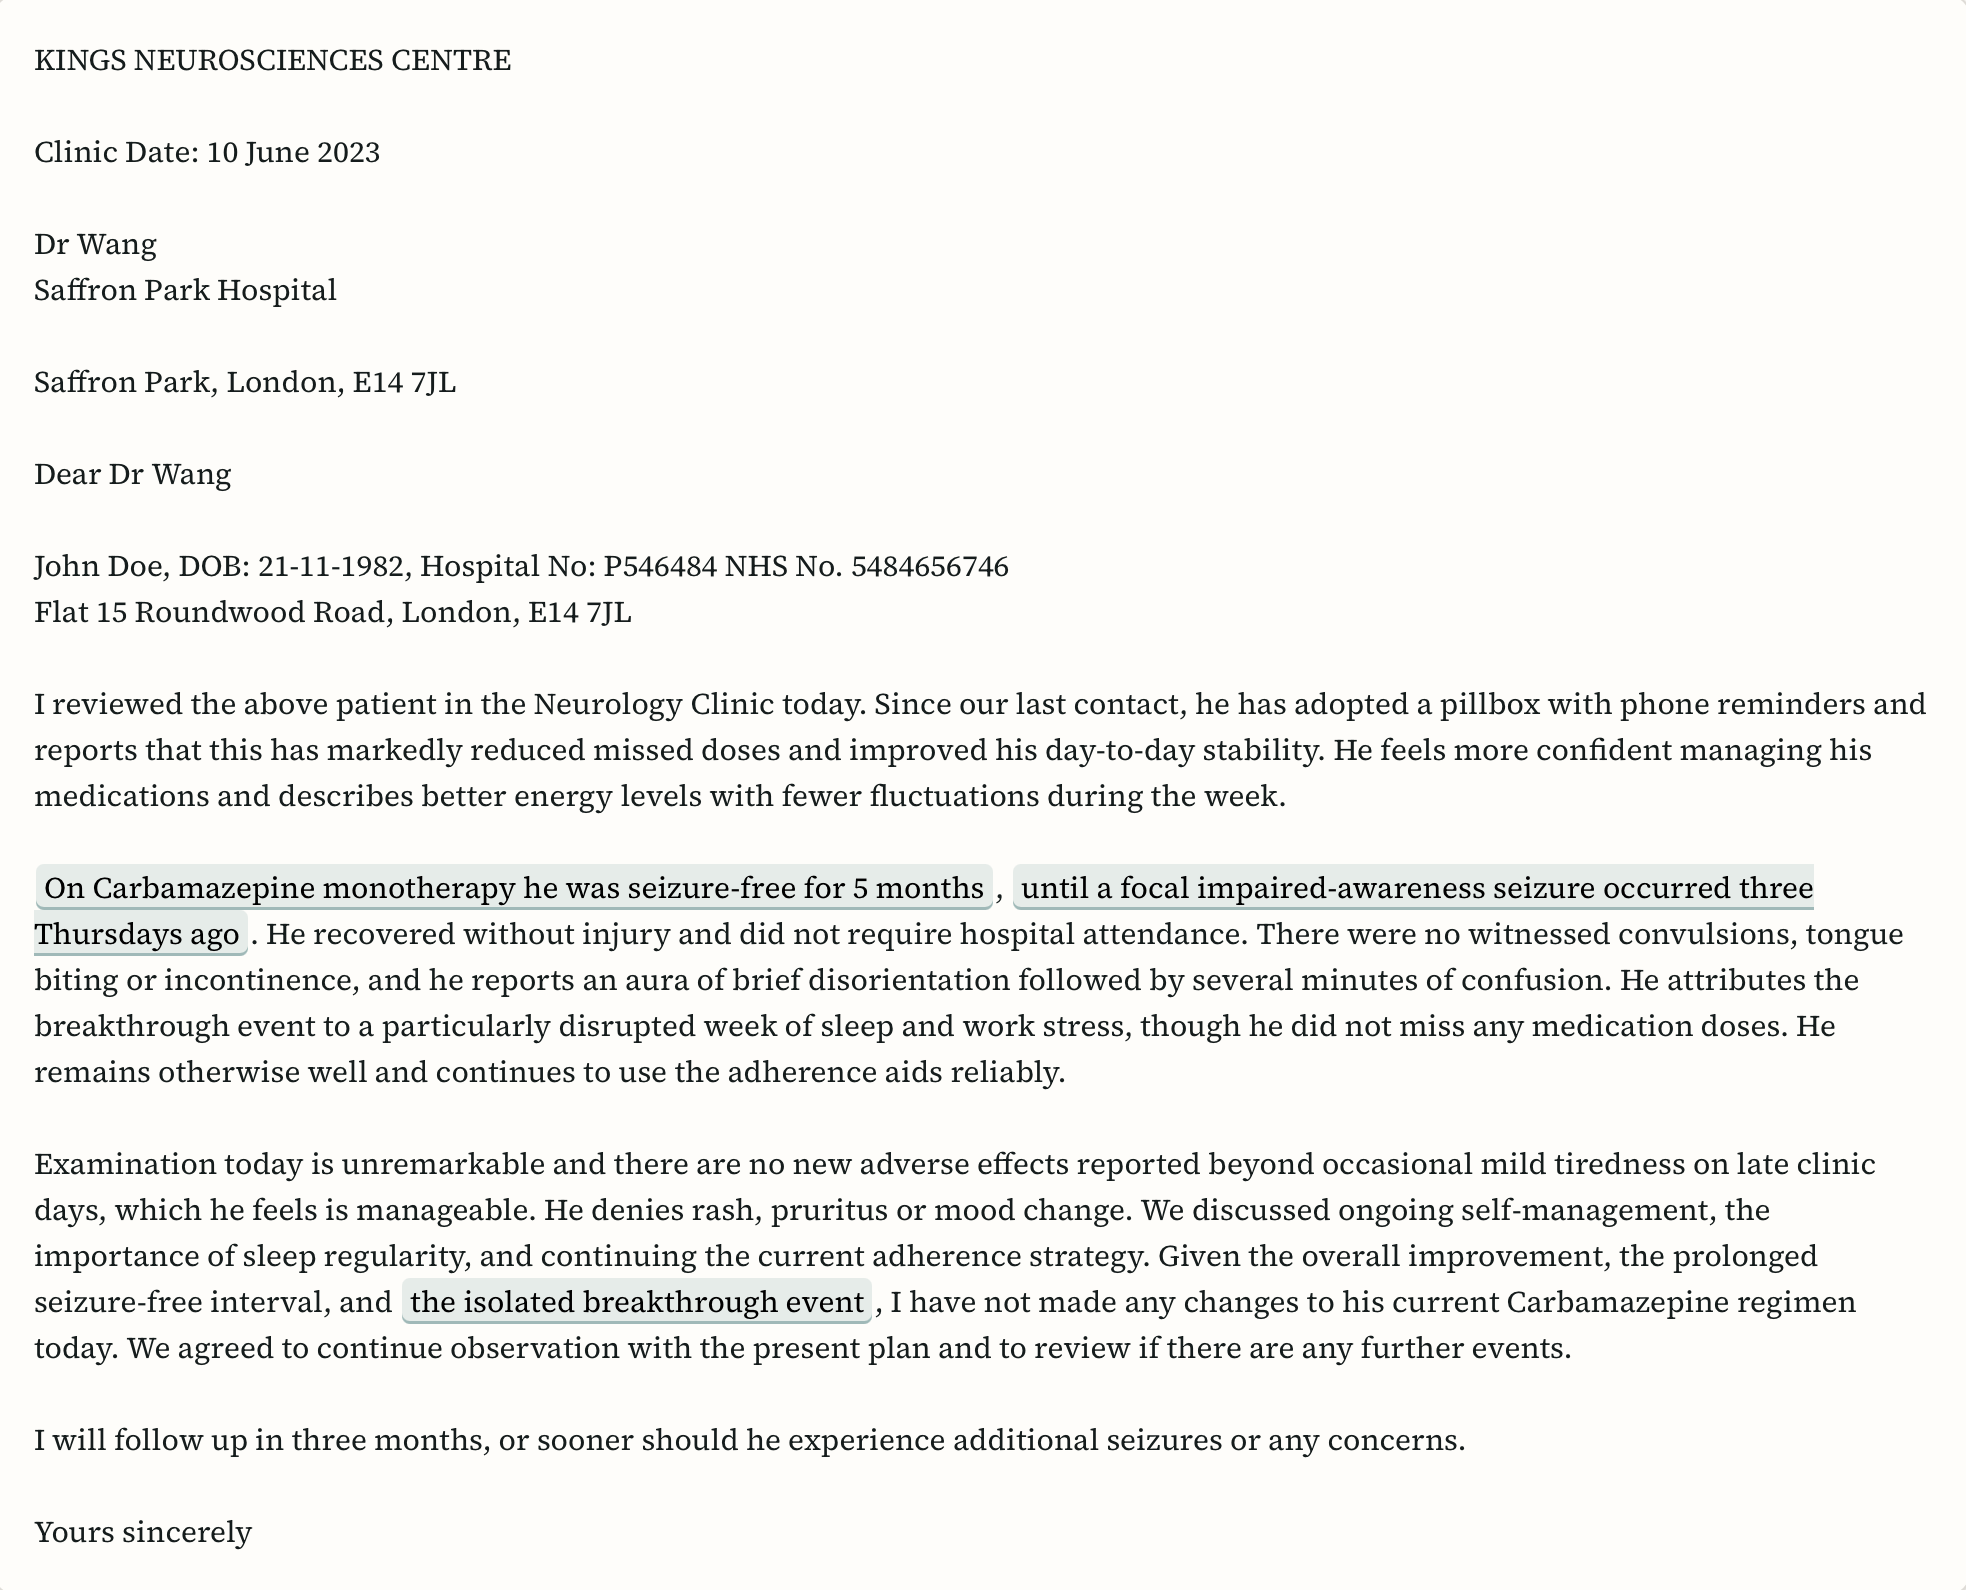
\includegraphics[width=\linewidth]{fig2.png}
    \caption{A clinic letter passes through three stages in the pipeline - recognise, encode and select - to generate structured labels with the exact text used from the letter to produce the label. Each of the three stages can be configured to use an LLM, rules or both. The example shown is the task of extracting a single label representing the patient's current seizure frequency burden.}
    \label{fig2}
\end{figure*}

\begin{table}[!t]
\caption{Pipeline configurations}
\label{tab:pipeline}
\centering
\begin{tabularx}{\linewidth}{Yccc}
\toprule
\textbf{Configuration} & \textbf{Recognise} & \textbf{Encode} & \textbf{Select} \\
\midrule
Rules only & Rules & Rules & Rules \\
LLM + Rules & LLM & LLM + Rules & Rules \\
LLM only & LLM & LLM & LLM \\
\bottomrule
\end{tabularx}
\end{table}

The development set was used to optimise the two key 
elements of the pipeline: the LLM prompt instructions and 
the rules. The focus of the optimisation process was to 
improve accuracy while . Qualitative error analysis was 
conducted to diagnose the cause of poor performance 
in particular areas and identify common error modes. 
Hypotheses were developed and tested to tune the 
prompt and rules iteratively. 

Through iterative error analysis on both the LLM and 
the rules, it became apparent that the complexity of the 
task was often a function of competing rules and 
guidelines. Often, improving a rule or a prompt 
instruction to address one class of error would harm 
another area because annotation policies are complex.
This complexity is a challenge for human annotators 
also; Fonferko-Shadrach \emph{et al.} described seizure
frequency as the most difficult category to annotate
and their inter-annotator agreement of 0.47 shows 
annotators often disagreed about how to represent
seizure frequency statements.

Decomposing the task into three stages allowed for 
cleaner separation of the policies on which types of 
facts to extract and which criteria to apply to exclude
specific variants of them. Decomposing the task into
three stages also made it possible to evaluate the 
performance at each individual stage and identify the 
bottlenecks in the system. It is this combination of 
a cleaner task decomposition for the pipeline and a
clearer view into the pipeline that enabled steady,
incremental gains to materialise from the optimisation
process.

\subsection{Evaluation}

To enable a direct comparison with the results in Gan \emph{et. al},
the pipeline is evaluated using the same micro-F1 score. They 
calculate the F1 on two categories; a fine-grained 'purist' score
and a coarser 'pragmatic' score. The more precise purist F1 is 
the primary metric in this paper, but the pragmatic F1 score is 
used for frequency bands with very small sample sizes (\textless20). A 
full specification of the categories is in Table 3. The rationale for 
categorising labels is so that semantically identical phrases 
are matched when exact labels differ, so that daily, once per day 
and every day would be considered correct matches to the gold
label '1 per day'. This evaluates the model on how effectively
it can identify the correct frequency rather than replicate 
precise phrasing. Further explanation on the categories can be
found in the original paper from Holgate \emph{et. al}.

The pipeline is evaluated on a held-out test set of 450 letters.
These letters were never used to tune prompts, rules or any 
other aspect of the pipeline. The test set is therefore used to 
evaluate how effectively the model generalises to unseen 
data. These results are compared against the evaluation set 
labelled Synthetic (1,166) in Gan \emph{et. al} which was 
also a held-out sample from the synthetic dataset, distinct 
from the training set used to fine-tune the models. It is 
important to note that Gan\emph{et. al} also tested their results 
a distinct set of real clinic letters to demonstrate generalisation 
to real data; our results and comparisons are limited purely to 
the synthetic data.

\begin{table}[!t]
\caption{Seizure frequency categories: Purist and Pragmatic}
\label{tab:categories}
\centering
\begin{tabularx}{\linewidth}{Ycc}
\toprule
\textbf{Purist} &
\textbf{Monthly rate} &
\textbf{Pragmatic} \\
\midrule
Daily & $\geq$30 & \multirow{4}{*}{Frequent} \\
More than weekly, less than daily & 16.6 & \\
Once a week & 4.0 & \\
More than monthly, less than weekly & 2.5 & \\
\midrule
Once a month & 1.05 & \multirow{4}{*}{Infrequent} \\
More than 6 months, less than monthly & 0.59 & \\
Once every 6 months & 0.17 & \\
Less than once every 6 months & 0.08 & \\
\midrule
Unknown & 1000 & Unknown \\
No seizure  frequency reference & 0 & No seizure \\
\bottomrule
\end{tabularx}

\vspace*{8pt}
\begin{minipage}{\linewidth}
\raggedright\footnotesize
Monthly rate is the midpoint of the purist category range normalised to the number of seizures per month. Originally defined in Holgate \emph{et. al}.
\end{minipage}
\end{table}

The primary objective of this research is to identify which 
component performs best at which stage. Table 2 shows 
the 3 pipeline configurations used in the evaluation: rules
at every stage, the LLM at every stage or a combination
of LLM and rules. For each configuration we evaluated 
the pipeline at each stage: recognise, encode and select.
This will produce a 3x3 matrix of results that answer two
key questions: 

\begin{enumerate}
\item Among the three pipeline configurations, which performs
best: rules, LLM, or a combination of both?
\item How much incremental value is there from the additional
encode and select stages?
\end{enumerate}

The primary hypothesis is that a combination of an LLM
plus rules will perform better than either on their own, 
because they have complementary strengths and those 
strengths are particularly well suited to distinct stages in
the pipeline. The secondary hypothesis is that multiple 
discrete stages will improve performance for the LLM,
regardless of whether the subsequent stages are rules or 
additional LLM calls. This builds on the idea that task 
decomposition is an effective form of context engineering, 
and is particularly useful in scenarios where the prompt 
is long and contains many layers of instructions. 

\section{Results}
\subsection{Development Environment}

Experiments using local language models took place on a 
Dell XPS 16 9640 running Windows 11, with an Intel Core 
Ultra 9 185H, 32 GB RAM, and an NVIDIA GeForce RTX 
4070 Laptop GPU (8 GB VRAM). Ollama v0.32.15 was 
used to serve the models. Two models were run on local 
hardware (Qwen 3.8 27b, Gemma 4 26B). 

Experiments using hosted APIs were were run from a Mac 
mini M1 with 16 GB unified memory on macOS 26.5.2. API
calls were made directly to the provider (OpenAI, DeepSeek) 
or through model routers (OpenRouter, AI Gateway) Four 
hosted models were used (Gemini 3.7 Flash, GPT 5.6 Luna, 
Grok 4.6, DeepSeek v4 Flash). 

All models used a temperature of 0 except Luna, which only 
accepts a temperature of 1. An ablation was run on Grok 
using a temperature of 1. All models used a thinking or effort 
level of 'low'. An ablation was run on Gemini using thinking
levels of medium and high. 

Python 3.14.4 was used to write the program. DSPy 3.2.1, 
Pydantic 2.13.4 and LiteLLM 1.87.1 were utilised as core
packages. DSPy was used to co-ordinate the model calls
and require structured JSON output. Pydantic was used
to validate the structured output conforms to the specified
schema. LiteLLM was used to deliver API calls to Ollama 
and the model routers.

\subsection{Benchmark Performance}

The combined LLM and rules pipeline achieved a purist 
micro-F1 score of 0.83, significantly higher than both 
rules only (0.71) and LLM only (0.79). It also exceeds the 
prior benchmark performance of 0.81 in Gan \emph{et. al} 
set by a model that was fine-tuned and evaluated using 
this same dataset of synthetic letters. While that is the only
paper to evaluate the same dataset with the same metric, 
Table 5 includes a summary of all 7 papers that reported 
a seizure frequency extraction score this decade. This 
pipeline is competitive with the best methods to date.

\begin{table}[!t]
\caption{Comparisons to past seizure frequency papers}
\label{tab:frequency}
\centering
\begin{tabularx}{\linewidth}{Yccc}
\toprule
\textbf{Author} & \textbf{Year} & \textbf{Method} & \textbf{F1 score} \\
\midrule
Xie et al. & 2022 & Fine-tuned LM & 0.83$^\ast$ \\
Decker et al. & 2022 & Rules & 0.82$^\ast$$^\ast$ \\
Fonferko-Shadrach et al. & 2024 & Rules & 0.66 \\
Fernandes et al. & 2024 & Fine-tuned LM & 0.37 \\
Holgate et al. & 2024 & Llama 2 & 0.73 \\
Holgate et al. & 2025 & Fine-tuned LLM & 0.68 \\
Gan et al. & 2026 & Fine-tuned LLM & 0.79 \\
\midrule
Brown \& Gan & 2026 & LLM + rules & 0.83 \\
\bottomrule
\end{tabularx}

\vspace*{8pt}
\begin{minipage}{\linewidth}
\raggedright\footnotesize
$^\ast$Drops to 0.73 on texts with a frequency statement.
$^\ast$$^\ast$Drops to 0.4 on external test set. 
\end{minipage}
\end{table}

This pipeline is particularly effective at identifying 
high frequency seizure events. A common theme in 
previous papers is that their method performed 
best when the task was predicting  'unknown' or  
'no seizures'. Xie et. al reported an F1 score of 0.92 on 
texts that contained no seizure frequency statement and 
0.73 when there was a seizure frequency reported. Gan 
et al. and Holgate et. al both report unknown as their 
highest scoring category at 0.89 and 0.87 respectively, 
while daily frequency (0.7, 0.41) and more than weekly 
(0.68, 0.55) are much lower. In this pipeline, daily (0.92) 
and more than weekly (0.91) are the best performing 
categories, significantly above unknown (0.74). 



\subsection{Recognise, Encode and Select Performance}


\subsection{Model Comparison}

6 Models

Thinking 

Temperature

The task is tightly defined with explicit schema and output 
requirements which limits the variation in model outputs 
linked to higher temperatures.

\subsection{Error Analysis}

The pipeline performed worst at predicting infrequent 
seizure events, mirroring the pattern in Gan et. al. The F1 
score for the infrequent (monthly or less) category was 
0.72 in this pipeline. This represents an improvement vs. 
0.67 in Gan et. al, but significantly worse performance 
vs. the pipeline's score of 0.95 on the frequent category. 


\section{Discussion}

This sensitivity to higher frequencies make it a particularly 
useful tool to identify patients with the greatest disease 
burden. This could be used in a number of settings. It could
be used in clinical care it could flag patients with a seizure 
burden above a typical threshold for the clinician's attention. 
It could be used in cohort selection to identify patients to be 
enrolled in clinical trials for a new medication or to be 
recommended for surgery. It could be used to build a 
phenotypic profile of patients to be used in retrospective 
analyses to understand how these patients differ from the 
average. Finally, it could be used as an outcome variable in 
predictive models to identify patients likely to experience 
frequent seizures and recommend an early intervention. 

\section{Conclusion}


\section*{References}

Please number citations consecutively within brackets \cite{b1}. The 
sentence punctuation follows the bracket \cite{b2}. 

\begin{thebibliography}{00}
\bibitem{b1} B. Fonferko-Shadrach \emph{et al.}, ``Using natural language processing to extract structured epilepsy data from unstructured clinic letters: development and validation of the ExECT (extraction of epilepsy clinical text) system,'' \emph{BMJ Open}, vol.~9, no.~4, 2019, Art.~no.~e023232.
\bibitem{b2} B. Fonferko-Shadrach \emph{et al.}, ``Annotation of epilepsy clinic letters for natural language processing,'' \emph{J. Biomed. Semantics}, vol.~15, no.~17, 2024.
\bibitem{b3} Y. Gan \emph{et al.}, ``Reproducible synthetic clinical letters for seizure frequency information extraction,'' arXiv:2603.11407, 2026.
\bibitem{b4} K. Xie \emph{et al.}, ``Extracting seizure frequency from epilepsy clinic notes: a machine reading approach to natural language processing,'' \emph{J. Amer. Med. Informat. Assoc.}, vol.~29, no.~5, pp.~873--881, 2022.
\bibitem{b5} B. Holgate, J. Davies, S. Fang, J.~S. Winston, J.~T. Teo, and M.~P. Richardson, ``Fine-tuning LLMs to extract epilepsy seizure frequency data from health records,'' in \emph{Proc. 24th Workshop on Biomedical Language Processing (BioNLP)}, 2025, pp.~44--55.
\bibitem{b6} S. Fu \emph{et al.}, ``Clinical concept extraction: A methodology review,'' \emph{J. Biomed. Informat.}, vol.~109, 2020, Art.~no.~103526.
\bibitem{b7} R. Grishman and B. Sundheim, ``Message Understanding Conference-6: A brief history,'' in \emph{Proc. 16th Int. Conf. Computational Linguistics (COLING)}, 1996, pp.~466--471.
\bibitem{b8} Y. Wang \emph{et al.}, ``Clinical information extraction applications: A literature review,'' \emph{J. Biomed. Informat.}, vol.~77, pp.~34--49, 2018.
\bibitem{b9} K. Xie, B. Litt, D. Roth, and C.~A. Ellis, ``Quantifying clinical outcome measures in patients with epilepsy using the electronic health record,'' in \emph{Proc. BioNLP Workshop}, 2022, pp.~369--375.
\bibitem{b10} M. Agrawal, S. Hegselmann, H. Lang, Y. Kim, and D. Sontag, ``Large language models are few-shot clinical information extractors,'' in \emph{Proc. Conf. Empirical Methods in Natural Language Processing (EMNLP)}, 2022, pp.~1998--2022.
\bibitem{b11} L. Chiticariu, Y. Li, and F. Reiss, ``Rule-based information extraction is dead! Long live rule-based information extraction systems!,'' in \emph{Proc. Conf. Empirical Methods in Natural Language Processing (EMNLP)}, 2013, pp.~827--832.
\bibitem{b12} B.~M. Decker \emph{et al.}, ``Development of a natural language processing algorithm to extract seizure types and frequencies from the electronic health record,'' \emph{Seizure}, vol.~101, pp.~48--51, 2022.
\bibitem{b13} interoperability-standard-contract
\end{thebibliography}

\vspace{12pt}

\end{document}
